\documentclass{article}

\usepackage[legalpaper, margin=1in]{geometry}
\usepackage{url}
\usepackage{booktabs}
\usepackage{amsmath}
\usepackage{graphicx}
\usepackage{chngcntr}
\usepackage{hyperref}
\usepackage{booktabs}
\usepackage{tabularx}
\usepackage{subfig}
\usepackage{longtable}
\usepackage{dblfloatfix}
\usepackage{listings}
\usepackage{placeins}
\usepackage{float}
\usepackage[dvipsnames]{xcolor}
\usepackage[style=ieee]{biblatex}

\addbibresource{refs.bib}
\DeclareCiteCommand{\citetitle}
{\boolfalse{citetracker}%
	\boolfalse{pagetracker}%
	\usebibmacro{prenote}}
{\ifciteindex
	{\indexfield{indextitle}}
	{}%
	\printtext[bibhyperref]{\printfield[citetitle]{labeltitle}}}
{\multicitedelim}
{\usebibmacro{postnote}}

\counterwithin{figure}{section}
\hyphenation{op-tical net-works semi-conduc-tor}


\begin{document}

\newcommand{\titleName}{Midterm - Design of a Heat Exchanger}
\newcommand{\courseName}{ME-407: Computational Fluid Dynamics}
\newcommand{\dateCreated}{\today}
\newcommand{\professorName}{Professor Bondi}

\begin{titlepage}
	\newcommand{\HRule}{\rule{\linewidth}{0.5mm}}
	\center
	\textsc{\LARGE Cooper Union for the Advancement of Science and
		Art}\\[1.5cm]
	{\color{teal} \HRule\\[0.4cm]}
	{\huge\bfseries \titleName\\[0.5cm] \textmd{\LARGE \courseName}}\\[0.4cm]
	{\color{teal} \HRule\\[0.4cm]}
	\begin{minipage}{0.4\textwidth}
		\begin{flushleft}
			\large
			\textit{Authors:}\\
			\textsc{Michal Meiner} \\
			\textsc{Preston Xu} \\
			\textsc{Benjamin Meiner} \\
			\textsc{Neil Sawhney} \\
		\end{flushleft}
	\end{minipage}
	~
	\begin{minipage}{0.4\textwidth}
		\begin{flushright}
			\large
			\textit{Professor:}\\
			\textsc{\professorName}

		\end{flushright}
	\end{minipage}
	\vfill\vfill\vfill
	{\large\dateCreated}
	\vfill
	%----------------------------------------------------------------------------------------

	\newpage
	\tableofcontents
\end{titlepage}

\title{\titleName}

%%%%%%%%%%%%%%%%%%%%%%%%%%%%%%%%%%%%%%%%%%%%%%%%%%%
%%%%%%%%%%%%%%%%%%%%%%%%%%%%%%%%%%%%%%%%%%%%%%%%%%%
\section{Objective}

%%%%%%%%%%%

\subsection{Model Assumptions}

%%%%%%%%%%%%%%%%%%%%%%

\section{Ballpark Hand Calculations}
To verify the CFD results to follow, ballpark hand calculations must be performed.

%%%%%%%%%%%

\subsection{Inlet Duct}

%%%

\subsubsection{Velocity Drop Over the Length of the Model}
The minimum velocity of 20 mph will be used at the inlet to ensure the worst case scenario is considered.

If we assume the flow is incompressible we can use conservation of mass to calculate the output velocity as shown in \autoref{eq:velocity-inlet_duct}. Because the inlet area is equal to the outlet area, the average velocity at the outlet is equal to the velocity at the inlet.

\begin{equation}
	\begin{aligned}
		A_1 V_1  & = A_2 V_2             \\
		V_2      & = \frac{A_1 V_1}{A_2} \\
		         & = \frac{A_1 V_1}{A_1} \\
		         & = V_1                 \\
		\Delta V & = 0
	\end{aligned}
	\label{eq:velocity-inlet_duct}
\end{equation}

%%%

\subsubsection{Pressure Drop Over the Length of the Model}

From the Darcy-Weisbach equation\cite{professional_engineer} the frictional head loss across the duct is given by \autoref{eq:darcy_weisbach}
\begin{equation}
	h_f = \frac{f L V^2}{2gD}
	\label{eq:darcy_weisbach}
\end{equation}

where
\begin{quote}
	\begin{description}
		\item[$f$] = the Moody, Darcy, or Stanton friction factor and is a function of $Re$ and $\frac{\epsilon}{D}$
		\item[$D$] = hydraulic diameter of the duct
		\item[$L$] = length over which the pressure drop occurs
		\item[$g$] = acceleration due to gravity
		\item[$\epsilon$] = roughness factor for the duct
	\end{description}
\end{quote}

\begin{figure}[h]
	\centering
	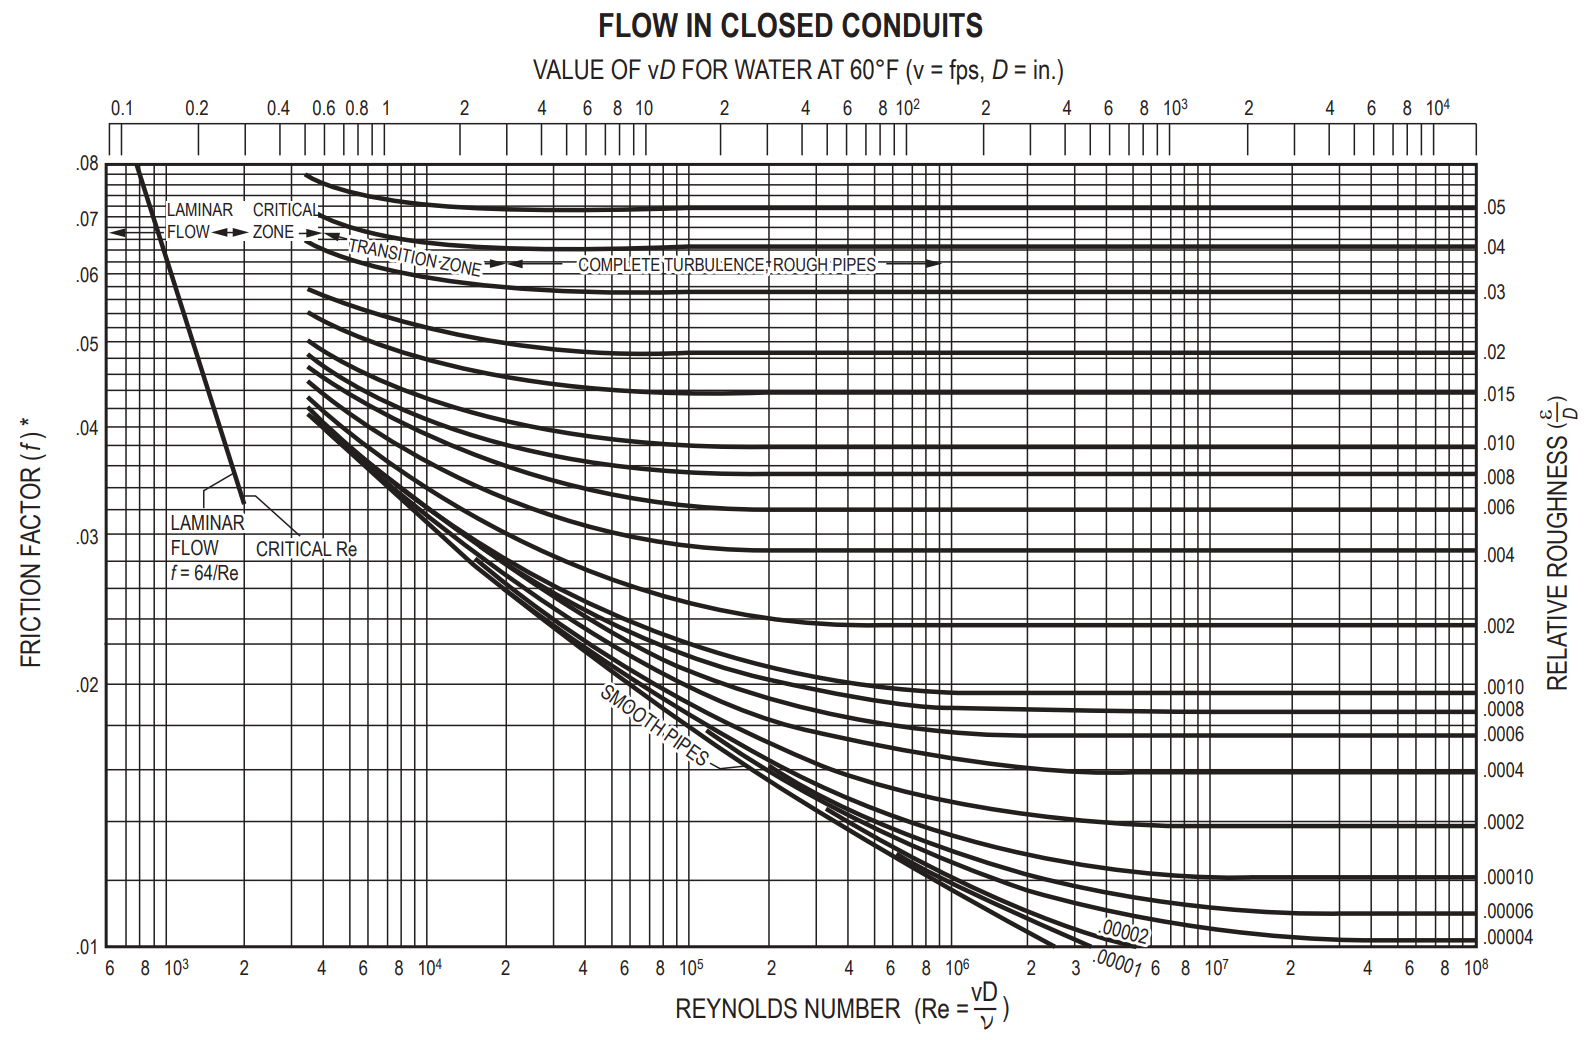
\includegraphics[width=0.5\linewidth]{img/hand_calcs/moody_diagram.png}
	\caption{Moody Diagram from \citetitle{professional_engineer}}
	\label{fig:moody_diagram}
\end{figure}

To find the friction factor, the Reynolds number must be calculated using \autoref{eq:reynolds-inlet_duct}. However, because the cross-section is not circular the hydraulic diameter must be calculated as shown in \autoref{eq:hydraulic_diameter}.

\begin{equation}
	\begin{aligned}
		D_h & = \frac{4A}{P}                                    \\
		    & = \frac{4*(10 in)*(20 in)}{2*(10 in) + 2*(20 in)} \\
		D_h & = 13.333 in
	\end{aligned}
	\label{eq:hydraulic_diameter}
\end{equation}

Now the Reynolds number can be calculated using \autoref{eq:reynolds-inlet_duct}. The density and dynamic viscosity of air at the worst case temperature of 108 $^\circ F$ is 0.070 lb/ft$^3$ and $0.01918$ cP respectively according to \citetitle{engineering_toolbox}.

\begin{equation}
	\begin{aligned}
		Re & = \frac{\rho V D}{\mu}                                      \\
		   & = \frac{(0.070 lb/ft^3)*(20 mph)*(13.333 in)}{(0.01918 cP)} \\
		Re & = 177014.265
	\end{aligned}
	\label{eq:reynolds-inlet_duct}
\end{equation}

The friction factor can now be found using the Moody chart from the \citetitle{professional_engineer} as shown in \autoref{fig:moody_diagram}. The pipe is assumed to be perfectly smooth, which yields a friction factor of 0.016. The pressure drop can then be calculated using \autoref{eq:pressure_drop}. Importantly, the friction factor assumes that the flow is fully developed, which it is not in this case. However, the pressure drop is only being used as a ballpark figure to compare to the CFD results, so this assumption is acceptable.

The head loss due to friction is then calculated using \autoref{eq:head_loss-inlet_duct} where the length over which the pressure drop occurs is measured from the center path line of the geometry to be 66.648 in.

\begin{equation}
	\begin{aligned}
		h_f & = \frac{f L V^2}{2D}                                                 \\
		    & = \frac{0.016*(66.648 in)*(20 mph)^2}{2*(32.174 ft/s^2)*(13.333 in)} \\
		h_f & = 12.834 in
	\end{aligned}
	\label{eq:head_loss-inlet_duct}
\end{equation}

The minor losses from the bend will also be considered. The head loss due to the bend is given by \autoref{eq:head_loss-bend}. The loss factor $K$ is obtained from \citetitle{engineering_toolbox} to be 0.5 for a 45$^\circ$ rounded bend. Although the bend is only 30$^\circ$, using the loss factor for a 45$^\circ$ bend will give a more conservative estimate.

\begin{equation}
	\begin{aligned}
		h_b & = K \frac{V^2}{2g}                         \\
		    & = 0.5 \frac{(20 mph)^2}{2*(32.174 ft/s^2)} \\
		h_b & = 80.23 in
	\end{aligned}
	\label{eq:head_loss-bend}
\end{equation}

The pressure drop is then calculated using \autoref{eq:pressure_drop}.

\begin{equation}
	\begin{aligned}
		\Delta P & = \gamma (h_f + h_b)                                    \\
		         & = (0.070 lb/ft^3)*(32.174 ft/s^2)(12.834 in + 80.23 in) \\
		\Delta P & = 0.0038 psi                                            \\
	\end{aligned}
	\label{eq:pressure_drop}
\end{equation}


%%%%%%%%%%%

\subsection{Heat Exchanger}

%%%%%%%%%%%%%%%%%%%%%%%%%%%%%%%%%%%%%%%%%%%%%%%%%%%

\section{Geometry}

%%%%%%%%%%%%%%%%%%%%%%%%%%%%%%%%%%%%%%%%%%%%%%%%%%%

\section{Mesh}

%%%%%%%%%

\subsection{Mesh Quality}

%%%%%%%%%%%%%%%%%%%%%%%%%%%%%%%%%%%%%%%%%%%%%%%%%%%

\section{Model Setup in Fluent}

%%%%%%%%%%%

\subsection{Boundary Conditions}

%%%%%%%%%%%%%%%%%%%%%%%%%%%%%%%%%%%%%%%%%%%%%%%%%%%

\section{Convergence}

%%%%%%%%%%%%%%%%%%%%%%%%%%%%%%%%%%%%%%%%%%%%%%%%%%%

\section{Results}

%%%%%%%%%%%%%%%%%%%%%%%%%%%%%%%%%%%%%%%%%%%%%%%%%%%

\section{Final Remarks}

%%%%%%%%%%%%%%%%%%%%%%%%%%%%%%%%%%%%%%%%%%%%%%%%%%%
%%%%%%%%%%%%%%%%%%%%%%%%%%%%%%%%%%%%%%%%%%%%%%%%%%%
\FloatBarrier

\nocite{*}
\printbibliography

% \begin{appendices}
% \end{appendices}

\end{document}